\chapter{Conversational Question Answering}
\label{chapter:conversation}

Chapters~\ref{chapter:factoid} and~\ref{chapter:non-factoid} focused on improving the answer retrieval performance for different types of user information needs.
However, question answering is not a one-way communication, where a user is only responsible for issuing requests and a system has to generate answers.
This setup is quite limited because it does not provide any means for the user to affect the behavior of a question answering system except by issuing new questions.
Similarly, it does not allow QA systems to request any additional information from the user, nor learn from the previous interactions.

Proliferation of mobile devices and more ``natural'' interfaces~\cite{hearst2011} are changing the way people search for information on the web.
Many experts envision that search in the near future will be a dialog between a user and an intelligent assistant, rather than just ``ten blue links'' in response to a one-shot keyword query.\footnote{\url{http://time.com/google-now/}} 
Participants of the SWIRL'2012 workshop foresaw a fusion of traditional IR and dialog systems~\cite{swirl2012}: ``Dialogue would be initiated by the searcher and proactively by the system.
The dialogue would be about questions and answers, with the aim of refining the understanding of questions and improving the quality of answers.''
Today we can witness this trend embodied in such products as Amazon Alexa, Google Home, Microsoft Cortana, Apple Siri, and others.

This chapter presents the research towards designing better conversational search interfaces.
Section~\ref{section:conversation:user-study} describes the user study we performed to learn how people use dialogs for information seeking scenarios and how the experience with modern personal assistants compares to a human-to-human dialog.
Sections~\ref{section:conversation:hints} and~\ref{section:conversation:clarq} focus on two particular interaction strategies, which allows a QA system to help the user either formulate or clarify their questions.

The contributions of the research described in this chapter are:
\begin{itemize}
\item A user study on conversational search, which provides actionable feedback on what people expect from such systems, how the expectations towards an automatic system differ from those towards humans, and what are some of the problems with using existing commercial personal assistants.
This work will be presented at CHI 2017 conference~\cite{vtyurina2017convsearch}.
\item A study of the effect of strategic hints, that a system might provide to the user, on search experience and success rate for complex informational tasks.
This work has been published as a short paper at SIGIR 2014~\cite{savenkov2014hint}.
\item An extensive analysis of clarification questions on community question answering platforms, and a model to predict the subject of a popular type of clarification questions, which shows the potential of such an approach.
This results were published in CHIIR 2017 conference proceedings~\cite{braslavski2017clarq}.
\end{itemize}

% =============================== User Study ===========================
\section{Conversational Search With Humans, Wizards, and Chatbots}
\label{section:conversation:user-study}

Chatbots and conversational assistants are becoming increasingly popular.
However, for information seeking scenarios, these systems still have very limited conversational abilities, and primarily serve as proxies to existing web search engines.
In this section, we ask: what would conversational search look like with a truly intelligent assistant?
To begin answering this question empirically, we conduct a user study, in which 21 participants are each given 3 information seeking tasks to solve using a text-based chat interface.
To complete each task, participants conversed with three conversational agents: an existing commercial system, a human expert, and a \textit{perceived} experimental automatic system, backed by a human ``wizard'' behind the curtain.
The observations and insights of our study help us understand the aspirations of users and the limitations of the current conversational agents -- and to sharpen a frontier of work required to improve conversational assistants for search scenarios.

\subsection{Motivation}
\label{section:conversation:user-study:motivation}

Personal assistants, such as Amazon's Alexa, Google Home, \etc are becoming increasingly popular, and people are integrating them in everyday life, \eg for simple tasks like setting up a timer, checking the calendar, requesting the latest news, a song, etc.\footnote{\href{url}{https://arc.applause.com/2016/09/26/amazon-echo-alexa-use-cases/}}.
The popularity of text-based chatbots is also on the rise in many areas of the web~\cite{ferrara2014rise}.
Most of them are template-based and are designed to fulfill a single, often monotonous, job~\cite{clement2015interacting,edwards2014bot}.
At the same time, a growing proportion of web search queries is formulated as natural language questions~\cite{aula2010does,liu2012web,pang2011search}, which is partially explained by the increasing usage of voice interfaces~\cite{white2015questions}.
Alas, for information seeking scenarios, existing chatbots and intelligent assistants are usually implemented as simply a ``proxy'' to existing web search engines, even though question-answering technology has made dramatic progress handling such question-like queries~\cite{tsai2015web}.
Furthermore, conversation provides additional opportunities to improve search quality. For example, a conversational system should be able to ask clarification questions~\cite{braslavski2017clarq} to better identify searcher's intent, and incorporate explicit user feedback~\cite{radlinski2017} -- something that is not normally available in a traditional web search scenario.
However, before jumping into implementing additional features for conversational search systems, it is important to gain a better understanding what the users' expectations are when interacting with a truly intelligent conversational search agent. It is equally important to anticipate how users might behave when faced with a conversational search system since behavioral feedback is critical for system evaluation and improvements. To this end, we explore the following research questions:

\begin{itemize}[noitemsep]
\item \textbf{RQ1}: What are the main expectations from a conversational search system?
\item \textbf{RQ2}: What are the differences between human-to-human and human-to-computer conversations?
\item \textbf{RQ3}: What characteristics prevent existing conversational agents from becoming effective tools for complex information seeking?
\end{itemize}

As no truly intelligent conversational search systems exist yet, we explore these research questions with a mixture of survey methods and user studies.
In the user study, the participants are faced with 3 complex information search tasks, derived from TREC Session track tasks~\cite{sessionTrack2014Overview}.
To eliminate the voice recognition quality variable, we chose to use text messaging as the interface between a participant and conversational systems.
We use three different conversational systems answering user requests: an existing commercial intelligent assistant, a human expert and a human disguised as an automatic system.
The results of our exploration suggest:
(1) people do not have biases against automatic conversational systems, as long as their performance is acceptable;
(2) existing conversational assistants are not yet up to the task, \ie they cannot be effectively used for complex information search tasks;
(3) by addressing a few requests from users that we identified, even current search systems might be able to improve their effectiveness and usability, with feasible modifications. 

\subsection{Study design}
\label{section:conversation:user-study:design}

\begin{figure}[h!]
	\centering
	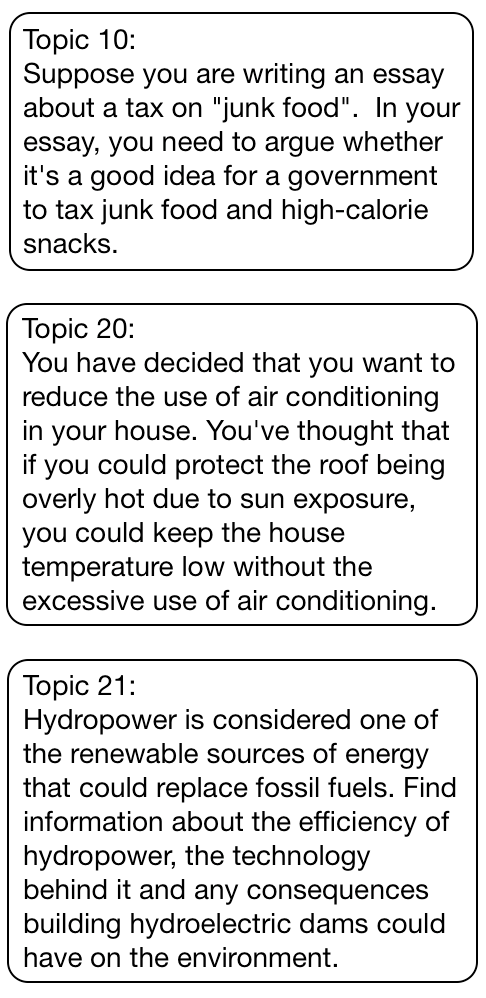
\includegraphics[width=0.4\textwidth]{img/FramedTopicsLeftAlign}
	\caption{Description of the tasks used in the user study on conversational search. All the tasks were obtained from TREC Session track 2014~\cite{sessionTrack2014Overview}.}
	\label{figure:conversation:user-study:tasks}
\end{figure}

We recruited 21 participants (graduate and undergraduate students at Emory University), to complete 3 different complex search tasks, taken from the TREC Session track 2014~\cite{sessionTrack2014Overview} (Figure~\ref{figure:conversation:user-study:tasks}).
The participants were asked to use an assigned text messenger-based conversational agent.
They were not given any instructions on how to use the agent and therefore were free to interact with it in any way they chose.
They were allowed to spend up to 10 minutes working on each task, after which they were asked to move on a topical quiz, consisting of 3 questions, designed for the topic.
After seeing the topical quiz questions, the participants were not allowed to talk to the agent anymore.
By doing so we ensured that the task stayed exploratory in nature, \ie the participants did not have a set of predefined points to cover.
After completing a topical quiz, the participants filled out a preference questionnaire, where they were asked to rate their experience with the agent, provide feedback about advantages and disadvantages of the agent.
After completing all tasks they filled out a final questionnaire.
The communication was implemented through the Facebook Messenger interface\footnote{\href{url}{http://www.messenger.com}}.
Participants used a Facebook account created specifically for the purpose of the study.
Message history was cleared prior to every experiment.

\subsubsection{Wizard agent}
\label{section:conversation:user-study:design:wizard}
Our first research question explores human behavior in human-computer communication.
There are currently no general purpose intelligent conversational search systems, that we could use for our purposes.
Therefore we ``faked'' one by substituting the backend with a person.
However, the participants were told that it was an experimental \textit{automatic} system, thus following a general Wizard-of-Oz setup.
We will be further referring to this system as the Wizard agent, and the person in the backend as the Wizard.
The Wizard had done the research about the topics of the 3 tasks prior to the experiment and compiled a broad set of passages covering most of the aspects of each topic.
At the time of the experiment, the Wizard tried to find the best passage to reply to the participant's question/comment.
However, in cases where such passage could not be found, the Wizard would reply with a passage retrieved from web search, or write a new passage.
In case the participant's question or comment was ambiguous, the Wizard was allowed to ask a clarification question to better identify the information need of the participant.
Our Wizard agent was allowed to maintain the context of the conversation, respond to vague questions, understand implied concepts, and provide active feedback in form of clarification questions when needed (all of these capabilities do not yet exist in commercial systems).
At the same time, by partially restricting the Wizard to a pre-compiled set of passages, we could maintain some consistency of answers between participants, \ie for the same question any participant would receive the same answer.
By analyzing the ways the participants communicated with the Wizard agent, we could gain insights about strategies people use in a human-computer dialogue for solving complex tasks and look for design implications for automatic conversational systems.

\subsubsection{Human agent}
\label{section:conversation:user-study:design:human}
To answer our second research question, about the differences between human-to-human and human-to-computer communication, we devised our second conversational agent -- the Human agent.
In this case, the Wizard from the previous setup was still serving as a backend, but the participants were explicitly informed that they were talking to a live person.
Another difference was that the Human agent was restricted to the pre-retrieved set of passages, but was free to slightly reformulate or revise the passages to better respond to the question.
By including both the Human and Wizard agents in the study, we were able to maintain a constant level of intelligence for both agents, thus comparing not the accuracy of each agent, but rather the participants' attitude and expectations towards a perceived automatic agent compared to a known human.

\subsubsection{Automatic agent}
\label{section:conversation:user-study:design:google}
For a comparison with an existing conversational agent, we used the Google Assistant\footnote{\href{url}{https://assistant.google.com/}} as a backend for our third agent.
Every message sent by a participant was forwarded to the Google Assistant app, and the response was forwarded back to the participant.
Most of the time, the response consisted of an URL and a text snippet. The participants were told that they were interacting with another experimental conversational system, but were not given any specific information about it.
By using a system representative of the state-of-the-art technology, we were able to evaluate its drawbacks, and situations where it failed to respond properly.

\subsection{Results}
\label{section:conversation:user-study:results}

After running the study, we analyzed message logs, answers to topical quizzes, and preference questionnaires and found the most popular trends and answers.
This section describes our findings in detail.
\begin{table}
  \centering
    \begin{tabular}{l*{4}{c}r}
    Agent                      & Human & Wizard & Automatic \\ 
    \hline
    Overall satisfaction       & 4.1 & 3.8 & 2.9 \\ 
    Able to find information   & 1.5 & 1.3 & 1.0 \\ 
    Topical quiz success       & 1.6 & 1.6 & 1.3 \\
    \end{tabular}
  \caption{Statistics on user satisfaction and success rates with human, wizard and automatic agent in conversational search user study.}
  \label{table:conversation:user-study:results}
\end{table}

\subsubsection{Overall satisfaction}
After completing each task participants rated their overall experience of working with each agent on a 1 to 5 Likert scale.
Average ratings for each agent are shown in Table~\ref{table:conversation:user-study:results}.
The differences in ratings of Human vs. Automatic systems, and the Wizard vs. Automatic systems were statistically significant (p $<$ 0.0001 and p $<$ 0.0005 respectively), while the difference between the Human vs. Wizard systems was not significant.
In the final questionnaire, after completing all the tasks, participants were asked which system they liked the most.
Out of 21 people, 8 people preferred the Human agent, 6 -- the Wizard agent, 4 -- the Automatic agent, 2 people said they would use the Wizard or the Human depending on their goals, and 1 person said he would choose between the Human and the Automatic agent depending on her goals.

\subsubsection{Able to find information}
Participants were asked whether they were able to find all the information about the topic they were looking for.
We coded each answer on a 0-2 scale (0 - no, I couldn't; 1 - partially; 2 - yes, I found everything I needed).
Average results for each agent are shown in Table~\ref{table:conversation:user-study:results}.

\subsubsection{Topical quiz success}
After completing each task participants were also asked 3 questions about the topic. We evaluated those questions on a scale 0-2, where 0 meant no answer, 1 - poor answer, 2 - good answer.
On average, participants showed a similar level of success with each agent.
The average user ratings for each agent are shown in Table~\ref{table:conversation:user-study:results}.

These results confirm our initial intuition that human-to-human conversation is more natural for the open-ended problem of the complex search task, compared with automatic conversational agents. This could be because people have experience talking to other people, and the results match their initial expectations. On the other hand, for any system that people have no experience with, they have to learn its functionality and ways to interact with it effectively.

We now turn to qualitative results, reporting the comments participants provided in the post-study questionnaire. The participants' comments broke down into the areas of maintaining context, trustworthiness, and social burden.

\subsubsection{Maintaining context}

\begin{figure}
    \centering
    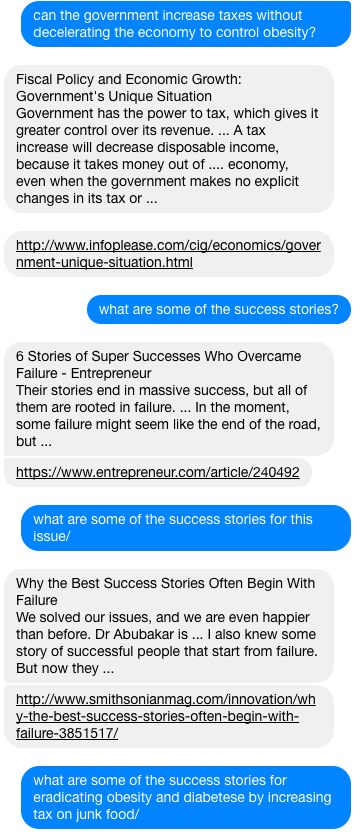
\includegraphics[width=0.5\textwidth]{img/conversation_userstudy_context}
    \caption{Automatic system (gray background) fails to maintain context, which causes the participant 15 (blue background) to reformulate his question twice.}
    \label{figure:conversation:user-study:context}
\end{figure}

\textit{Participant 19 (P19): ``It didn't use contextual information so there was no way to expand on the previous answer it gave me.''} Within a conversation, people expect that the main topic of the discussion is maintained, and they tend to ask short questions, omitting the subject, or referring to the subject using pronouns. Formulating a full question takes effort and is unnatural. For the Automatic system, anaphora resolution did not always work, which annoyed the participants. Similarly, when dealing with the Human and Wizard systems, participants pointed out the ease of use, because their partially stated questions were understood, and relevant answers were returned (Figure~\ref{figure:conversation:user-study:context}).

\subsubsection{Trustworthiness of the sources is crucial}

\begin{figure}
    \centering
    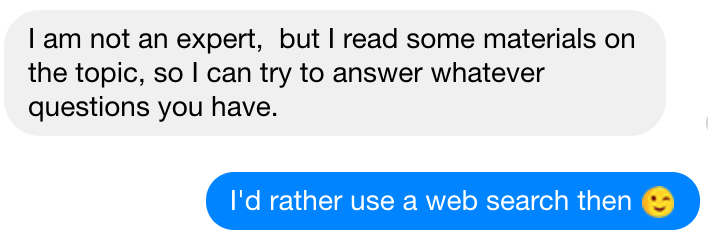
\includegraphics[width=0.5\textwidth]{img/conversation_userstudy_prefersearch}
    \caption{A participant prefers web search to talking to a person. Part of a conversation between participant 7 (blue background) and Human agent (gray background).}
    \label{figure:conversation:user-study:prefersWebSearch}
\end{figure}

\textit{P7: ``I ... like to be able to verify the credibility of the sources used.''} Even though the Automatic system did not always respond with a relevant result, it received approval from our participants for providing sources of its answers. Out of 21 participants, 13 people said that being able to access the URL allowed them to assess the trustworthiness of the source and therefore to accept or reject the answer. On the other hand, in spite the Human and Wizard systems returning more relevant results, they were both criticized for not providing the sources (Figure~\ref{figure:conversation:user-study:prefersWebSearch}).

\subsubsection{Social burden}

\begin{figure}
    \centering
    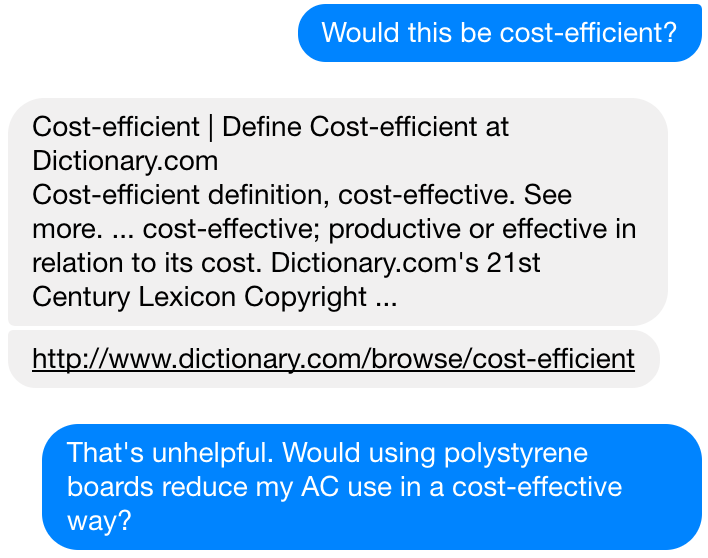
\includegraphics[width=0.5\textwidth]{img/FullExample1}
    \caption{Explicit user feedback could be used to recover from failure. Part of a conversation between participant 12 (blue background) and Automatic system (gray background).}
    \label{figure:conversation:user-study:feedback}
\end{figure}

\textit{P15: ``you have to think about social norms, asking too much, being too stupid, not giving them enough time to respond, troubling them.''} When dealing with the Human system, 4/22 participants reported that they felt uncomfortable talking to a person, thought more about the social norms, were afraid to ask too many questions, were not sure how to start and end a conversation. This additional burden of interacting with humans further motivates research in the area of automated conversational agents as the medium of choice for a notable fraction of use cases (Figure~\ref{figure:conversation:user-study:feedback}).


\subsection{Discussion and design implications}
\label{section:conversation:user-study:discussion}

Based on our findings we devised a list of recommendations for a conversational agent design, that according to our empirical study will improve user experience significantly.

\textbf{Context.}
Maintaining a context of the conversation to enable short questions and comments is crucial to user experience since formulating long sentences each time feels unnatural and takes longer.

\textbf{Provide sources of answers.}
Finding relevant and precise answers is important. But trustworthy sources are equally important, and their absence may diminish the credibility of the system. While the Automatic agent supported each answer with an URL, Human and Wizard did not, unless specifically asked. 
%This may have impacted the user satisfaction with the system, confirmed by anecdotal feedback from the participants.

\textbf{Use feedback.}
One crucial difference of conversational setup from web search is the ability of a user to provide the system with explicit feedback. It is likely to contain essential information that may help the system to get back up from failure and improve upon the previous result. 
%Feedback processing may also be of help in case a user decides to switch the focus of the search. It will also produce rich data for user satisfaction evaluation. \\

\textbf{Opinion aggregation.}
According to the participants, sometimes what is needed is the \textit{experience} of other people in similar situations.
A good conversational system should be able to aggregate opinions and present them to the user in a short summary, perhaps explaining each one. 
Participant 17 said: \textit{``It would be nice if I could see a summarization of different opinions that there exist -- from different sources.''}
% This is why they may prefer to talk to a friend -- to learn about the experiences of a knowledgeable trustworthy person or to get a broader view from the web.

\textbf{Direct answers vs. expanded information.}
For this aspect, our participants split into 2 camps: those who prefer getting direct answers to the question provided, and those who prefer also getting a broader context.
People from Camp 1 complained that the answers returned by the systems were too long (even for the Wizard and Human), and preferred to have their questions answered directly with minimum extra information.
Camp 2, on the other hand, said that they prefer talking to a person, who would recognize their true information need (beyond the immediate question) and provide the relevant information.


In this section, we investigated human behavior when using conversational systems for complex information seeking tasks.
We also compared participant behavior when talking to a human expert, vs. a perceived automatic system.
We observed that people do not have biases against automatic systems, and are glad to use them as long as their expectations about accuracy were met.
However, existing agents often fail to provide a reasonable response, and users often struggle with finding the right way to ask or reformulate a question.
In the next section, we will investigate search hints, which a system can provide to its users in order to help them solve complex informational search tasks.
%Future research directions include further investigating the possibilities for improving existing conversational agents and studying the effect of these changes on user experience. 


%======================= Search hints begin =======================

\section{Search Hints for Complex Informational Tasks}
\label{section:conversation:hints}

Some informational needs are more complex than others.
While existing technologies can handle relatively simple questions pretty well, they might leave users frustrated with their responses for more difficult requests.
Bilal and Kirby~\cite{Bilal:2002:DSI:637512.637516} reported that about half of the participants of their user study felt frustration when searching.
Xie and Cool~\cite{xie2009understanding} demonstrated that most of the time users have problems with formulating and refining search queries.
Besides good retrieval performance, a successful search requires users to possess certain skills.
Search skills can be trained, \eg Google offers a course\footnote{\href{url}{http://www.powersearchingwithgoogle.com}} on improving search efficiency.
Although very useful, such courses are time-consuming and detached from real search problems of these particular users.
Displaying search hints is another technique that has both learning effect and offers immediate assistance to the user in solving her current search task.
Moraveji et al.~\cite{Moraveji:2011:MIU:2009916.2009966} demonstrated that hints, suggesting certain search engine functionality, help people find answers more quickly, and the effect is retained after a week without hints.

In this section, I explore \textit{strategic} search hints, that are designed to guide a user in solving her search problem.
More specifically, for complex search tasks users might find it helpful to choose the divide-and-conquer strategy, \ie splitting an original difficult question into smaller problems, searching answers to the subtasks and combining them together.
Two sets of strategic hints were manually designed: \textit{generic} hints describing the divide-and-conquer strategy in general and \textit{task-specific} hints providing a concrete strategy to solve the current search task.
To evaluate the effect of the hints on behavior and search success we conducted a user study with 90 participants.
The results of the user study demonstrate that well-designed task-specific hints can improve search success rate.
In contrast, generic search hints, which were too general and harder to follow, may have the negative effect on user performance and satisfaction.

\subsection{User Study}
\label{section:conversation:hints:user-study}

\begin{figure}[t]
\centering
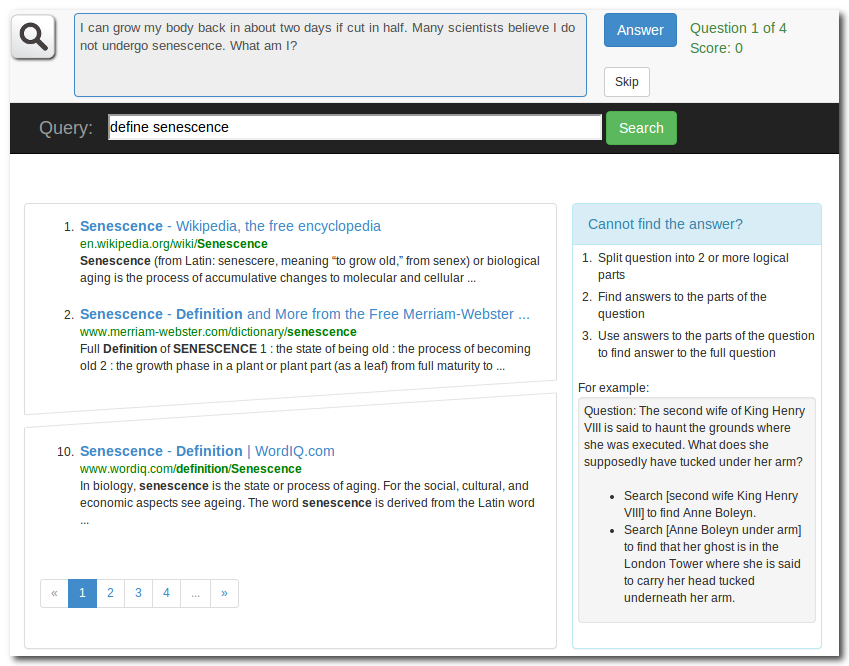
\includegraphics[width=\textwidth]{img/hints_ufindit}
\caption{The interface of the search game used in the study of the effect of strategic search hints on success in solving complex informational tasks.}
\label{figure:conversation:hints:ufindit}
\end{figure}

\begin{table}
\small
\centering
\begin{tabular}{r|p{4cm}|p{4cm}|p{4cm}}
& Question & Correct Answer & Specific hints \\
\hline
1 & I can grow body back in about two days if cut in half. Many scientists think I do not undergo senescence. What am I? & Senescence means ``biological aging''. Hydra is considered biologically immortal and regenerates fast. & \parbox[t]{4cm}{
1. Find what is senescence \\
2. Find who does not undergo senescence \\
3. Find who can also regenerate body and choose the one that satisfies both conditions} \\\hline
2 & Of the Romans "group of three" gods in the Archaic Triad, which one did not have a Greek counterpart? & Archaic Triad includes Jupiter, Mars, and Quirinus. Among those Quirinus did not have a Greek counterpart. &
\parbox[t]{4cm}{
1. Find the names of the gods from the Archaic triad\\
2. For each of the gods find a Greek counterpart
}\\ \hline
3 & As George surveyed the ``waterless place'', he unearthed some very important eggs of what animal? & "Gobi" in Mongolian means ``Waterless place''. The first whole dinosaur eggs were discovered there in 1923. & \parbox[t]{4cm}{
1. Find what is the ``waterless place'' mentioned in the question?\\
2. Search for important eggs discovery in this ``waterless place''}\\ \hline
4 & If you were in the basin of the Somme River at summers end in 1918, what language would you have had to speak to understand coded British communications? & Cherokee served as code talkers in the Second Battle of the Somme. & \parbox[t]{4cm}{
1. Find the name of the battle mentioned in the questions\\
2. Search for which coded communications language was used in this battle\\
} \\
\end{tabular}
\caption{Search tasks and specific search hints used for user study on the effectiveness of strategic hints for complex informational search tasks.}
\label{table:conversation:hints:tasks}
\end{table}

To estimate the effect of strategic search hints on user behavior we conducted a study in a form of a web search game similar to ``a Google a Day''\footnote{\href{url}{http://www.agoogleaday.com/}} and uFindIt \cite{Ageev:2011:FYG:2009916.2009965}.
Participants were hired using Amazon Mechanical Turk\footnote{\href{url}{http://www.mturk.com/}}.

The goal of the web search game was to find answers to several questions with the provided web search interface (Figure~\ref{figure:conversation:hints:ufindit}).
Players are instructed not to use any external tools.
The questions are given one by one and since tasks might be too difficult, a chance to skip a question was provided, although users were instructed that effort put into solving a question will be evaluated.
To answer a question each player needs to provide a link to a page containing the answer as well as its text.
The answer is automatically verified and a pop-up box notifies a player if the answer is incorrect (since the answer can be formulated differently, the presence of a keyword was checked).
A player can then continue searching or skip the question when she gives up.
A bonus payment was made to players who answer all questions correctly.
We used Bing Search API\footnote{\href{url}{https://www.microsoft.com/cognitive-services/en-us/bing-web-search-api}} as a back-end of the game search interface.
All search results and clicked documents were cached so users asking the same query or clicking the same page got the same results.
At the end of the game, a questionnaire was presented asking for feedback on user satisfaction with the game, prior experience, and other comments.

The tasks for the study were borrowed from the ``A Google a Day'' questions archive.
Such questions are factual, not ambiguous and usually hard to find the answer to a single query, which makes them interesting for user assistance research.
We filtered search results to exclude all pages that discuss solutions to ``A Google a Day'' puzzles.
To do this we removed pages that mention a major part of the search question or ``a google a day'' phrase.
To keep users focused throughout the whole game we limited the number of questions to 4.
The tasks are described in Table \ref{table:conversation:hints:tasks} and were presented to all participants in the same order to ensure comparable learning effects.

The questions have multiple parts and to solve them it is helpful to search for answers to parts of the questions and then combine them.
In one of the previous studies, we observed, that most of the users did not adopt the divide-and-conquer strategy, but kept trying to find the ``right'' query.
We decided to estimate the effect of strategic search hints, suggesting users to adopt the new strategy.

We built 2 sets of strategic hints: \textit{task specific} and \textit{generic}.
Task-specific hints described steps of one of the possible solutions to each question (Table \ref{table:conversation:hints:tasks}).
The second set contained a single hint, which was shown for all tasks. Generic hint described the divide-and-conquer strategy:\\

\hrule
\begin{enumerate}[noitemsep]
\item Split the question into 2 or more logical parts
\item Find answers to the parts of the question
\item Use answers to the parts of the question to find answer to the full question
\end{enumerate}

For example, the question: ``The second wife of King Henry VIII is said to haunt the grounds where she was executed. What does she supposedly have tucked under her arm?''
\begin{enumerate}[noitemsep]
\item Search [second wife King Henry VIII] to find Anne Boleyn.
\item Search [Anne Boleyn under arm] to find that her ghost is in the London Tower where she is said to carry her head tucked underneath her arm.
\end{enumerate}
\hrule
\vspace{5mm}

To control for the learning effect demonstrated in~\cite{Moraveji:2011:MIU:2009916.2009966}, each user was assigned to one of the three groups: (1) users who did not get any hints; (2) users who got task-specific hints; (3) users who got the generic hints.


\subsection{Results and Discussion}
\label{section:conversation:hints:results}

From 199 unique participants, who clicked the HIT on Amazon Mechanical Turk only 90 players finished the game.
We further examined all games manually and filtered out 9 submissions for one of the following reasons: lack of effort (\eg skipped several tasks after none or a single query) or usage of external resources (\eg the answer was obtained without submitting any queries or results explored did not contain the answer).
Furthermore, 10 players from the group which received hints indicated in the survey that they did not see them, so we filtered out those submissions and finally, we had 71 completed games (29 for no hints, 20 for task-specific hints and 22 for generic hints groups).

\textbf{Effects of Search Tips on Performance}.
In order to measure search success rate we looked at the number of questions answered correctly by different groups of users\footnote{Since users were allowed to skip a question we are counting the number of questions that were eventually solved correctly even if a player made some incorrect attempts.}.
Figure~\ref{figure:conversation:hints:task_success} shows that success rate is higher for users who saw task-specific hints compared to users who did not get such assistance.
Surprisingly, having the generic hint decreased the success rate, although users could easily ignore a hint they did not like.
A possible explanation is: generic hints were harder to follow and users who tried and failed became frustrated and did not restart their searches.

The plot of average time to answer a question on Figure~\ref{figure:conversation:hints:task_time} does not show an improvement for the task-specific hints group, except for the question 1.
Our task-specific hints represent a possible way to solve a problem and there is no guarantee, that it is the fastest one.
It is worth noting, that users from the generic search hint group had slightly higher variance in success time, which can probably be explained by the fact that some users were successful in finding the right way to follow the hint and some other users struggled with it much longer.
Another insight comes from the number of incorrect attempts users made.
Figure~\ref{figure:conversation:hints:incorrect} demonstrates the average number of incorrect answer attempts for all groups of users.
Although the variance is high, there is a tendency for users who saw task-specific hints to make fewer attempts than both other groups.
This is not in direct correspondence with time spent on the game.
It seems that the users who saw a clear strategy to solve the question were less likely to notice plausible, but incorrect solution.
Moreover, we analyzed texts of incorrect answers and can conclude that a big part of incorrect submission are due to users trying all possible options they found on the way, even if these options are clearly wrong.


\begin{figure}
\small
\centering
  \begin{subfigure}[t]{0.32\textwidth}
  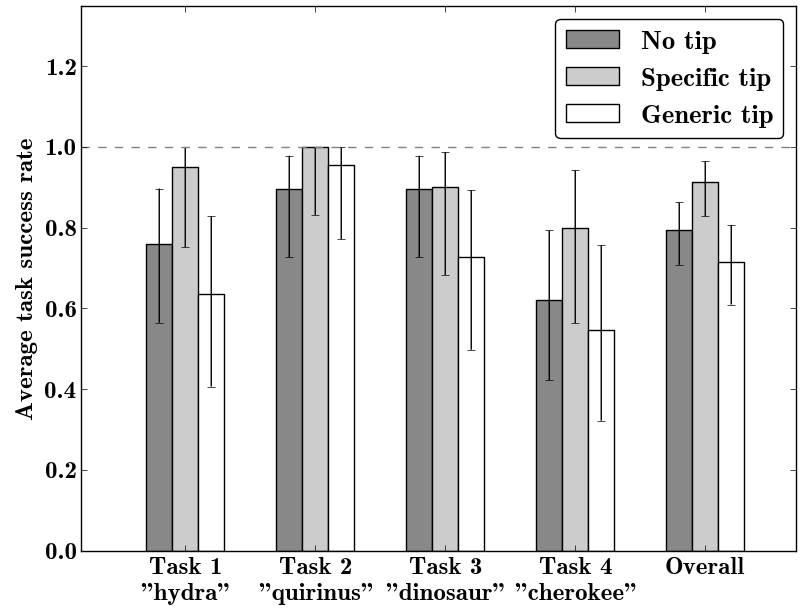
\includegraphics[width=\textwidth]{img/hints_success_per_task}
  \caption{Success rate per task for each group of participants}
  \label{figure:conversation:hints:task_success}
  \end{subfigure}
  \begin{subfigure}[t]{0.32\textwidth}
  \centering
  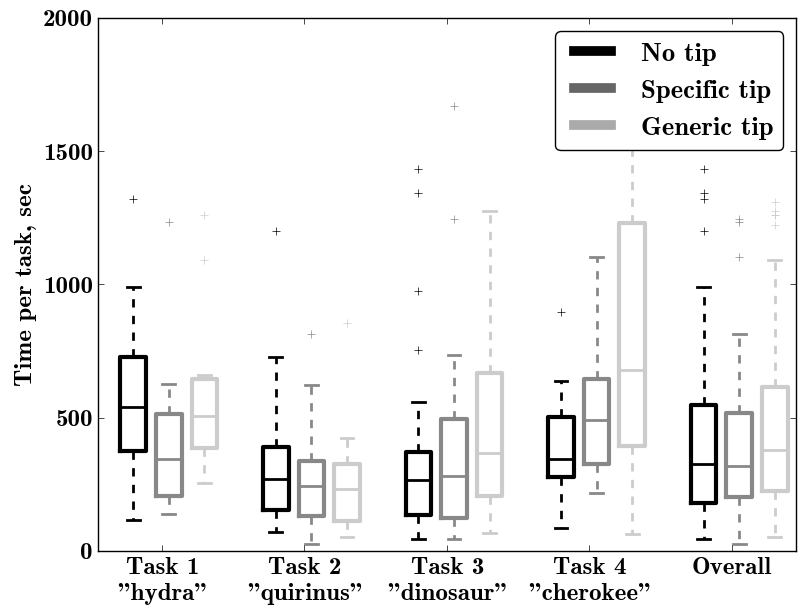
\includegraphics[width=\textwidth]{img/hints_time_per_task}
  \caption{Task completion time for each group of players}
  \label{figure:conversation:hints:task_time}
  \end{subfigure}
  \begin{subfigure}[t]{0.32\textwidth}
  \centering
  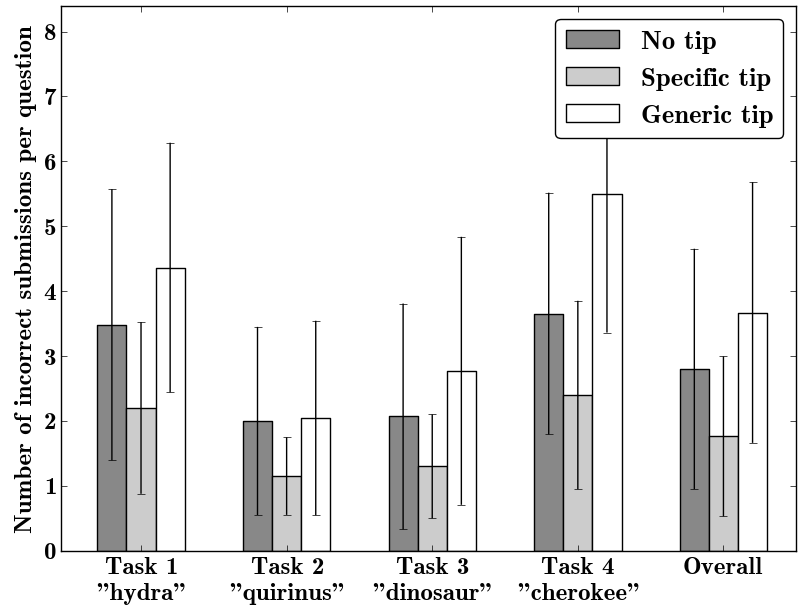
\includegraphics[width=\textwidth]{img/hints_incorrect}
  \caption{The number of incorrect submission attempts per question for all groups of users}
  \label{figure:conversation:hints:incorrect}
  \end{subfigure}
\caption{Results of the user study on the effectiveness of strategic search tips on search task success rate.}
\label{fig:conversation:hints:results}
\end{figure}

\begin{figure}[h]
\centering
\begin{subfigure}[t]{0.32\textwidth}
    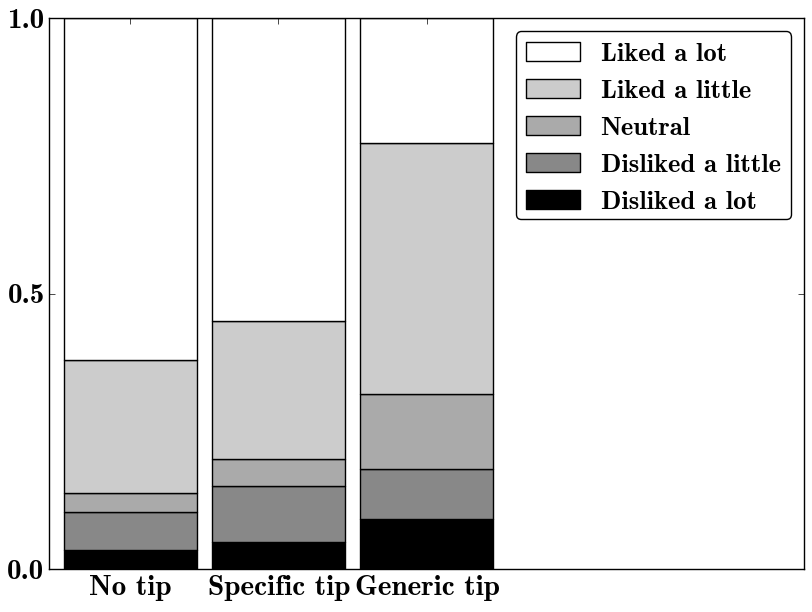
\includegraphics[width=\textwidth]{img/hints_liked}
    \caption{How did you like the game?}
    \label{figure:conversation:hints:survey:liked}
\end{subfigure}
\begin{subfigure}[t]{0.32\textwidth}
    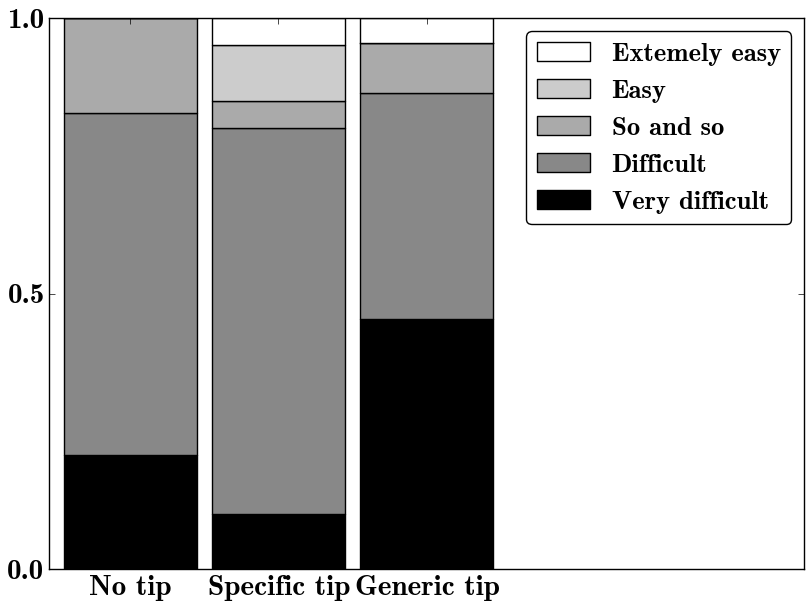
\includegraphics[width=\textwidth]{img/hints_difficult}
    \caption{How difficult was the game?}
    \label{figure:conversation:hints:survey:difficult}
\end{subfigure}
\begin{subfigure}[t]{0.32\textwidth}
    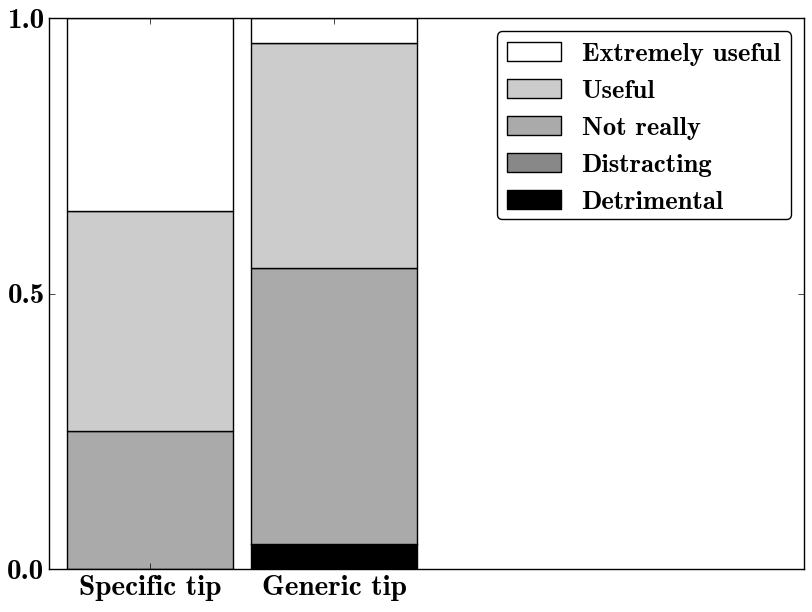
\includegraphics[width=\textwidth]{img/hints_useful}
    \caption{Were search hints useful to you?}
    \label{figure:conversation:hints:survey:useful}
\end{subfigure}
\caption{Proportions of replies to some of the survey question for each group of users.}
\label{figure:conversation:hints:survey}
\end{figure}

We also looked at other search behavior characteristics: number of queries submitted, the number of clicks made, the average length of the queries.
The variance in these characteristics was too high to make any speculations regarding their meaning.

\textbf{Effects of Search Tips on User Experience}.
Finally, we looked at the surveys filled out by each group of users.
Figure \ref{figure:conversation:hints:survey} presents proportions of different answers to three of the questions: ``How did you like the game?'', ``How difficult was the game?'' and ``Were search hints useful to you?''.
Surprisingly, user satisfaction with the game was lower for users who saw hints during the game and users who did not get any assistance enjoyed it more.
The replies to the question about game difficulty are in agreement with the success rate: users who saw task-specific hints rated difficulty lower than participants who struggled to find the correct answers.
The game was very difficult on average, however, some participants from the group who received task-specific hints surprisingly rated it as very easy, which suggests that our hints do help users.
This is supported by the answers to the last question on whether hints were helpful (Figure \ref{figure:conversation:hints:survey:useful}).

% To summarize, the results of the conducted user study suggest that specific search hints can be helpful, which is indicated by higher success rate, lower number of incorrect attempts and positive feedback at the end of study survey.
% In contrast, generic hints can have the negative effect on user experience, which is indicated by lower success rate, increased number of incorrect attempts and higher perceived tasks complexity according to the survey.

\subsubsection{Summary}
\label{section:conversation:hints:summary}

In this section, we studied the effect of strategic search hints on user behavior. 
The conducted user study in a form of a web search game demonstrated the potential of good hints in improving search success rate.
However, to be useful, they should be designed carefully.
Search hints that are too general can be detrimental to search success.
We also find that even searchers who are more effective using specific search hints, feel subjectively less satisfied and engaged than the control group, indicating that search assistance has to be specific and timely if it is to improve the searcher experience.

In addition to providing users with some hints on how to continue their search process, it is important for a QA system to improve question understanding skills.
Unfortunately, some questions contain certain ambiguity.
In conversational settings, a natural thing to do for such requests is to ask a clarification question, which is the focus of the next section of this dissertation.


% =================== Clarification questions : begin ======================

\section{Clarifications in Conversational Question Answering}
\label{section:conversation:clarq}

One key capability required to make conversational question answering effective is asking \textit{clarification questions} (\clarQ) proactively, when a user's intent is not clear, which could help the system provide more useful responses.
With this in mind, we make the first attempt to examine the clarification questions (\clarQ) that users ask on the Stack Exchange community question answering (CQA) platform.
We analyze Stack Exchange data in two domains
corresponding to about 300K questions and comments.
The contributions of this study are threefold:
\begin{itemize}[noitemsep]
\item To learn about user behavior associated with \clarQ and about their role in CQA communications. We find that \clarQ~are quite common on Stack Exchange, and therefore represent a good source of data for analysis.
\item To study the types of \clarQ~users ask in different situations. We classify clarification questions into several categories according to their target as well as syntactic patterns, which help define the space of \clarQ~for future research;
\item To make the first step towards automatic generation of \clarQ: 
we build a model to predict the subject of a popular type of clarification questions, which shows the potential of such approach for future research.
\end{itemize}

\subsection{Dataset Description}
\label{section:conversation:clarq:data}

\begin{figure}[t]
\centering
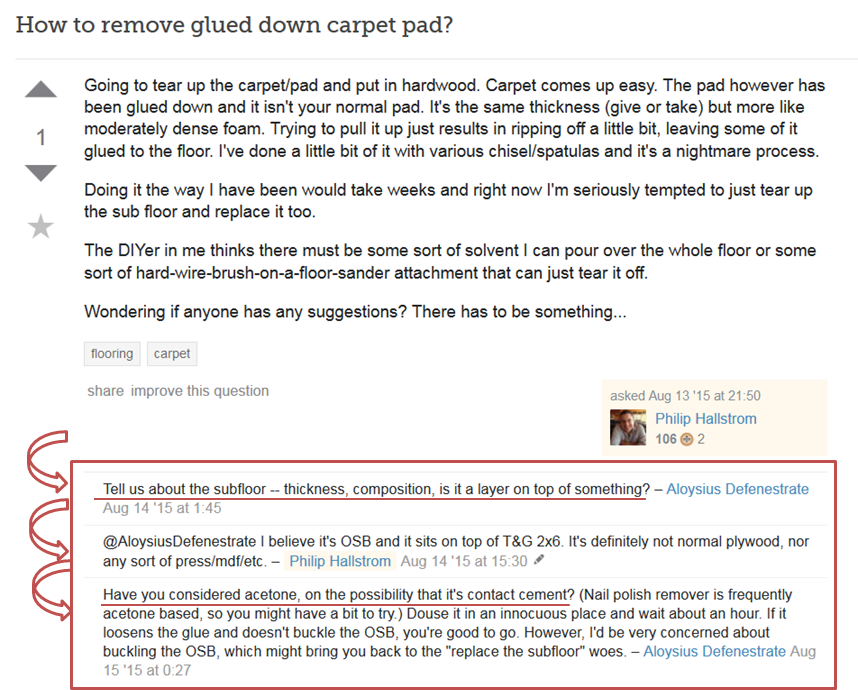
\includegraphics[width=0.95\textwidth]{img/diy}
\caption{Screenshot of a DIY question page from StachExchange CQA platform with threaded conversation in comments.}
\label{figure:conversation:clarq:diy}
\end{figure}

For our analysis we took two Stack Exchange sites -- Home improvements (DIY)\footnote{\href{url}{http://diy.stackexchange.com/}} and Arqade (GAMES)\footnote{\href{url}{http://gaming.stackexchange.com/}}.
These two domains are quite different -- the former is devoted to purely practical real-world problems, the latter -- to the virtual world of video games. Stack Exchange users can comment on the questions and answers;
sometimes it leads to multi-turn forum-like discussions (see Figure~\ref{figure:conversation:clarq:diy}).
The data dumps provided by Stack Exchange\footnote{\href{url}{https://archive.org/details/stackexchange}} cover a period of 5.5 years -- from July 2010 to January 2016. 

We define \clarQ~in a straightforward manner: sentences in comments to the initial questions ending with the question mark, provided by the users different from the asker of the initial question, four words and longer. This heuristic is not perfect, as clarification requests can be formulated as a declarative sentence, \eg \textit{Please provide details...} or question mark can be just missed. At the same time, these interrogative comments may be rhetorical questions, or not on the initial question's subject.
Nevertheless, manual inspection showed that this definition of \clarQ~is operational and allows extraction of \clarQ~ with precision acceptable for an exploratory study.

Basic statistics of the two datasets are reported in Table~\ref{table:conversation:clarq:data}.

\begin{table}[h]
\centering
\small
\begin{tabular}[t]{p{8cm}rr}
& \textit{DIY} & \textit{GAMES}\\
\hline
\# of questions & 20,702 & 62,511\\
\# of answers & 36,580 & 105,167\\
\# of accepted answers & 8,381 & 40,049 \\
\# of comments & 87,238 & 228,074\\
average question length in words & 130.8 & 86.5\\
average comment length in words & 33.8 & 25.8\\
\# of comments on questions & 37,296 & 96,247\\
\# of non-asker comments on questions & 27,873 & 72,495\\
\# of comments on questions with `?' & 11,040 & 21,448 \\
\clarQ~followed by asker's comments & 3,679 & 8,021 \\
\clarQ~followed by post editing & 4,270 & 9,038 \\
\clarQ~followed by post editing by asker & 1,631 & 3,772\\  
\end{tabular}
\caption{Statistics of the Stack Exchange datasets, used for the clarification questions study.}
\label{table:conversation:clarq:data}
\end{table}

\subsection{Results}
\label{section:conversation:clarq:results}

\subsubsection{User behavior}
\label{section:conversation:clarq:behavior}

As Table~\ref{table:conversation:clarq:data} shows, the presence of \clarQ~in CQA is substantial. Many characteristics such as questions/answers, accepted answers/all answers ratios are similar for both domains.
Questions and comments in DIY are longer then in GAMES, which is expected: DIY implies richer and more diverse contexts.
Askers are engaged in communication even after the initial question is posted: they comment on questions and edit them (however, questions are edited by community members more often).
Although there are more comments on questions in DIY, GAMES seem to be somewhat more conversational: askers respond to questions on questions more often.
Interestingly, thousands of initial questions are followed by clarifications, and in many cases, these are followed by the original question being edited, presumably in response to the clarification request. 

Unfortunately, we see that questions followed by \clarQ~do not differ much from questions without any comments in length -- a simple assumption that \clarQ~are targeted at short underspecified questions does not hold.
The hypothesis that questions asked by novice and less experienced community members (based on users' ratings) receive more \clarQ~is not supported either.
We also did not find any topical specificity of questions with \clarQ~based on tags. 

\begin{figure}
\centering
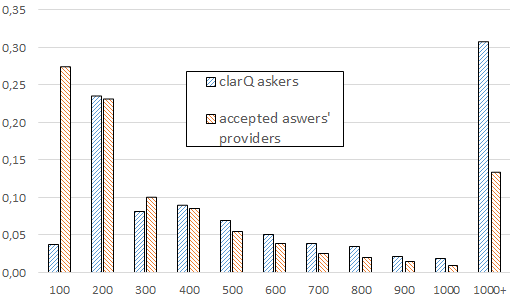
\includegraphics[width=.75\linewidth]{img/user_ratings.png}
\caption{Distribution of users' reputation scores in the groups of accepted answers' providers and commentators on questions (GAMES).}
\label{figure:conversation:clarq:users_scores}
\end{figure}

Figure~\ref{figure:conversation:clarq:users_scores} shows rating distribution of the GAMES users, who ask \clarQ~and those who provide accepted answers (i.e., the best answerers in the community).
We can observe that distribution for the former group is shifted towards higher scores (DIY exhibits a very similar distribution). 
However, the users who ask for clarifications provide answers for the initial questions very rarely. 
This observation suggests that \clarQ~in CQA are a form of `quality control measures' undertaken by most experienced users.


\subsubsection{Question types and patterns}
\label{section:conversation:clarq:types}

\begin{table}[h!]
\centering
\begin{tabular}[t]{lrl}
\textit{Category} & \textit{\%} & \textit{Example} \\
\hline
More Info & 28.6 & What OS are you using? \\
Check & 29.3 & Are you on a 64-bit system?\\
Reason & 8.5 & What is the reason you want a drip pan?\\
General & 10.2 & Can you add more details to this question?\\
Selection & 9.9 & Are you using latex or oil based Kilz?\\
Experience & 10.2 &  Have you tried to update video card drivers?\\
Not a \clarQ & 13.9 & Out of curiosity what elo are you? \\
\end{tabular}
\caption{The distribution of questions in StackExchange comments by type. Some comments contain several \clarQ of different types, so the sum is more the 100\%.}
\label{table:conversation:clarq:qtypes}
\end{table}

\begin{table}[h!]
	\centering
	\small
	\begin{tabular}[t]{p{4cm}rrp{5.5cm}}
		\textbf{Pattern} & \textbf{DIY} & \textbf{GAMES} & \textbf{Example} \\
		\hline
		\textit{have you tried}& 256 & 1,123 & Have you tried reinstalling the game yet?\\
		\textit{do you have}                 & 592 & 692 & Do you have enough disk space left?\\
		\textit{do you mean}                 & 248 & 552 & Do you mean a separate tub and shower? \\
		\textit{are you sure}                & 206 & 366 & Are you sure you have timber frame construction? \\
		\textit{what (is|are) the}             & 558 & 361 & What is the slope of the floor? \\
		\textit{what do you}                 & 103 & 284 & What do you mean by squeaking?\\
		\textit{(are|is) there any}            & 154 & 147 & Are there any airflow ducts in the room already?\\
		\textit{can you (post|provide)}     & 204 & 125 & can you post some pictures? \\
		\textit{how X (is|are)}                & 290 & 117 & how old is the water heater? \\
		\textit{is it a}                     & 186 & 112 & is it a constant 18-22 fps?\\
		\textit{what (kind|type) of}         & 344 & 106 & What kind of texture is on the wallpaper? \\
		\textit{why do you}                 &  73 & 101 & Why do you need to run it from the Flash drive?\\
		\textit{have you checked}             &  66 &  98 & Have you checked the frequency of the outlets? \\
		\textit{is it possible}             &  78 &  84 & Is it possible the tank is just over filling? \\
		\textit{do you know}                 & 120 &  64 & Do you know the manufacturer of the fixture?\\
	\end{tabular}
	\caption{Question patterns in comments (sorted by frequency in GAMES) from StackExchange dataset.}
	\label{table:conversation:clarq:patterns}
\end{table}


In order to investigate \clarQ~breakdown by type, we sampled 294 comments on questions from both domains, and two authors performed manual annotation analogously to~\cite{kato2013}, see results in Table~\ref{table:conversation:clarq:qtypes}.
Comments that are not aimed at clarifying the main question contain rhetorical or humorous questions,
questions to previous comments, citations of other questions on the platform, etc. Interestingly, the breakdown of \clarQ~by type is roughly the same as in~\cite{kato2013}.

Further, upon examining the sample we identified a list of common three-word question starting patterns, and calculated their frequency in the whole dataset, see Table \ref{table:conversation:clarq:patterns}. 
As can be seen from the Table~\ref{table:conversation:clarq:patterns}, some patterns are quite indicative for the clarification type (\eg \textit{what kind of} corresponds to \textit{More info} category, whereas \textit{have you tried} -- to \textit{Experience}).
This observation suggests that recognition of clarification question type is a feasible task.


\subsubsection{Clarification subject prediction}
\label{section:conversation:clarq:subj-prediction}

As we have shown, there are many different kinds of questions that users ask in comments.
Many of them address a certain ambiguity present in questions, \eg \textit{what kind of} questions inquire about a subtype of a mentioned object.
These questions are quite common (Table~\ref{table:conversation:clarq:patterns}) and have a simple structure, which makes them a quite appealing target for automatic question generation.
The first step for such question generation is to predict the object to ask about.
We collected questions, which received at least one \textit{what (kind|type) of} \clarQ~in DIY. 
From these comments and questions, we extracted noun phrases using Stanford CoreNLP parser~\cite{manning-EtAl:2014:P14-5}, and kept only those questions that have a common pair of noun phrases in the question and comment.
We formulated the task as the noun phrase ranking problem, where the noun phrase from the comment should be placed higher on the list than other noun phrases from the question.
Each candidate phrase was represented by the following set of features:
\begin{itemize}[noitemsep]
\item \textbf{prior}: number of times the noun phrase was used in comments (separate from the training and test sets)
\item \textbf{topicality}: number of occurrences of the phrase in the current question (in title and body together)
\item \textbf{position}: position of the first occurrence of the noun phrase relative to the beginning of the question
\item \textbf{entropy}: collection-based statistic, computed using all noun phrases that contain the given noun phrase, which estimates the number of different modifications of the current noun phrase object
\item \textbf{length}: number of words in the noun phrase
\end{itemize}

To train the ranking model we used a random forest algorithm implemented in the RankLib library\footnote{\href{url}{https://sourceforge.net/p/lemur/wiki/RankLib}}.
We optimized DCG@10 and Table~\ref{table:conversation:clarq:np_rank_performance} summarizes the performance metrics on 10-fold cross validation.
As we can see, even with a limited set of features our model was able to place the true subject of a clarification question above other candidates in 35\% of the cases.
To study the contributions of different feature groups we conducted a series of experiments to train the model with each group individually.
The results in Table~\ref{table:conversation:clarq:np_rank_performance} suggest, that the number of occurrences of a phrase and the position of the first occurrence are strong features, and confirms our intuition that \clarQ~are usually asked about the main topic of the question.
However, some noun phrases are more ambiguous in general, therefore the prior feature also contributed significantly to the quality of the model.

\begin{table}[h]
\centering
\begin{tabular}[t]{lrrrr}
\textit{Model} & \textit{P@1} & \textit{MAP} & \textit{RR@10} & \textit{ERR@10} \\
\hline
random & 0.077 & 0.215 & 0.231 & 0.015 \\
+ entropy & 0.143 & 0.334 & 0.350 & 0.024 \\
+ length & 0.148 & 0.337 & 0.345 & 0.024 \\
+ position & 0.165 & 0.335 & 0.357 & 0.024 \\
+ prior & 0.214 & 0.402 & 0.427 & 0.030 \\
+ topicality & 0.319 & 0.426 & 0.473 & 0.032 \\
all features & 0.350 & 0.508 & 0.549 & 0.038 \\
% random & 0.0769 & 0.2151 & 0.2305 & 0.0146 \\
% + entropy & 0.1425 & 0.3336 & 0.354 & 0.0244 \\
% + length & 0.1481 & 0.337 & 0.3498 & 0.024 \\
% + position & 0.1652 & 0.3346 & 0.3568 & 0.0237 \\
% + prior & 0.2137 & 0.4018 & 0.4266 & 0.03 \\
% + topicality & 0.3191 & 0.4255 & 0.4731 & 0.0315 \\
% all features & 0.3504 & 0.5078 & 0.5491 & 0.0381 \\
\end{tabular}
\caption{Performance metrics (P@1 -- precision at~1, MAP -- mean average precision, RR@10 -- reciprocal rank at 10, ERR@10 -- expected reciprocal rank) of the ranking model for ``ambiguous'' noun phrase selection problem.}
\label{table:conversation:clarq:np_rank_performance}
\end{table}

Overall, our experiment showed promising results for predicting the subject for a certain type of \clarQ.
As a next step, our model can be combined with an ambiguity detection classifier, which would trigger clarification as a response from a conversational search agent.

\subsection{Discussion}
\label{section:conversation:clarq:Discussion}

As a step towards general-purpose interactive QA system, we analyzed clarification questions asked by CQA users.
In particular, we examined user interactions related to \clarQ, as well as the role and place of these questions in  CQA.
We analyzed a large sample of \clarQ according to their type and identified most common syntactic patterns in a large collection of \clarQ.
Finally, we conducted an experiment aimed at automatically detecting the subject of clarification question of a particular type.

Based on our analyses, we can conclude that \clarQ~are common in CQA archives, and introduce a valuable resource for user behavior studies and QA research.
Clarification questions asked by community members are an important component in maintaining the quality of user-generated content in CQA.
Furthermore, we see that clarification questions are quite diverse in topic and style, are highly dependent on context and individual characteristics of the users.
However, there are several types of questions and syntactic patterns that are common within each domain.
As a first step towards automatically generating clarification questions, we show promising results on identifying the subject of \clarQ~based on a small set of shallow features.
Our findings suggest that CQA data may be useful for research in the field of interactive QA.

% There is still a long way to go towards automatic generation of clarification questions.
% This capability would require identification of user questions which are indeed ambiguous, choosing an aspect and type of clarification, and generate the text. 
% These steps imply naturally an analysis of answer candidates, which was not addressed in the current work. 
% A significant portion of \clarQ deals with properties, attributes, relations and types of the objects mentioned in the initial question.
% This suggests that domain-specific knowledge-based approach to \clarQ~generation can be promising. 
% These two tasks -- the use of candidate answers and knowledge bases -- define the directions for future research in the area of clarification questions generation for interactive QA.


% =================== Clarification questions : end ======================

\section{Summary}
\label{section:conversation:summary}

This Chapter described the research I have done on conversational question answering, which gives a system opportunities to exploit a rich set of possible interactions with its users.
First, I described the design and implications of the user study we conducted to investigate the current state in conversational search, and looked into what users expect from a dialog agent compared to a human interlocutor, and what is missing from an existing state-of-the-art commercial system.
We learned, that users do not have any prejudice towards automatic question answering agents, and for some people they are actually preferable, avoiding certain social norm issues.
We identified some directions for future research in order to move existing systems towards user expectations, by providing a diverse set of opinions as well as information sources, improving context maintenance techniques, and learning from user feedback.
As the first steps in these directions, I discussed search hints and clarification questions, which can be provided by the system to either help users structure their search process or clarify some of the ambiguities.
The results of the conducted research showed that hints tailored to a specific search problem can effectively guide the user through the search process.
However, generic hints might actually take away the feeling of control from the user and lower both satisfaction and success rate.
To study the phenomenon of clarification questions, we analyzed the data from one of the community question answering platforms and identified different types of clarifications, \eg ``what type of ...'' questions, that aim at requesting information on a particular type of an object mentioned in the question.
The model we built to predict the subject of such questions showed a reasonable performance, and demonstrate the potential of this approach for automatic clarification generation.

Together, the research described in this chapter provides desiderata for future developments in conversational search and question answering and shows promising first steps in some of these directions.